\documentclass[11pt]{article}

\usepackage{graphicx}
\usepackage{amsmath,amssymb}
\usepackage{url}

\usepackage{caption}
\usepackage{subcaption}
\usepackage{parskip}
\setlength {\marginparwidth }{2cm}  % needed to resolve issues
\usepackage{todonotes}
% \usepackage[toc,page]{appendix}
\usepackage{hyperref}

\usepackage[margin=1.5in,footskip=0.25in]{geometry}

%\newfontfamily{\cyrillicfonttt}{Liberation Mono}

% Margins
%\evensidemargin=0in
%\oddsidemargin=0in
%\textwidth=6.5in

%\setlength{\jot}{8pt}

% Information
\title{Investigating the Viability of Clustering Method in the BdG-formalism}
\author{Axel Tibbling}
\date{ }

\begin{document}

\maketitle

\section{Introduction}\label{sec:introduction}

Superconductivity is the quantum state of a material where all applied magnetic fields are expelled, with an interesting side feature where the electrical resistance goes to zero, effectively letting electrons pass without energy dissipation. Many have tried to mathematically describe this phenomena, and was done first at a macroscopical scale by the London brothers \cite{londonElectromagneticEquationsSupraconductor} 1935. But what happens at the microscopical scale? This is what Bardeen, Cooper and Schrieffer investigated in their paper \cite{bardeenTheorySuperconductivity1957} 1957, which lead to what is now known as Bardeen–Cooper–Schrieffer (BCS) theory. This has become a widely accepted microscopic theory of superconductivity, but is not in general solvable due to its quartic operator term creating/annihilating pairs of electrons. 

The solution to this came shortly after, developed by both Nikolay Bogoljjiubov and John George Valatin independently in 1958 \cite{valatinCommentsTheorySuperconductivity1958a,bogoljubovNewMethodTheory1958} . They found a solution to the homogeneous BCS problem by ismorphically transforming the particles to quasi particles, leaving the commutation relations invariant. This transformation is known as the \textit{Bogoljubov-Valatin transformation}, and is used to diagonalize the Hamiltonian. These quasiparticle states can be seen as representing whether a system is in a superconducting state or not.  

One can draw associations between the BdG numerical solution method with the Monte Carlo method. Both systems study the total energy of the whole system, and does this for the whole system. Some reserchers saw this as an inefficiency in the Monte Carlo method and realized that only local changes in energy may be considered, yielding positive results \cite{karmakarDisorderStabilizedBreachedpair2022, kumarTravellingClusterApproximation2006}.

In this study we employ a similar method for numerical analysis of the BdG Hamiltonian. In section \ref{sec:background} is the BCS model of choice introduced and relevant theory is discussed. Continuing to section \ref{sec:methods} is the normal numerical method for BdG given as well as the proposed cluster method. Results are the given in section \ref{sec:results} and discussed in section \ref{sec:discussion}.  


\section{Background and choice of model}\label{sec:background}

The BdG formalism has its origin in BCS theory, which will act as the starting point. This theory was the first theory to describe superconductivity at a microscopic level, and has been widely accepted in the scientific community as a fundamental description of superconductivity \cite{girvinModernCondensedMatter2019, sharmaReviewTheoriesSuperconductivity2015}. In its essence does it describe an attractive interaction between electrons dominating over the Coloumb force which one would naturally assume to repel electron pairs. 

Interacting electrons form a bounded state which is very stable and does not dissipate energy into the surrounding system. This is a notable observation, as it is one of the key characteristics of superconductors; that electrons does not dissipate their energy, which macroscopicly is seen as resistance.

\subsection{Model of choice}

The system chosen for study is a 1D spin-chain, where the BCS interaction is on-site, and the hopping matrix element is merely neraest neighbor. Chemical potential has also been included. The Hamiltonian for this system is chosen to be 

\begin{align}\label{eq:model}
	H = &-t \sum_{\langle i j\rangle, \sigma}\left(c_{i \sigma}^{\dagger} c_{j \sigma} + c_{j \sigma}^{\dagger} c_{i \sigma}\right) \nonumber \\ 
	    &- V \sum_j n_{j \uparrow} n_{j \downarrow} -\mu \sum_j\left(n_{j \uparrow}+n_{j \downarrow}\right) 
\end{align}

The number operator here is defined as

\begin{equation}
	n_{j, \sigma} = c_{j, \sigma}^\dagger c_{j, \sigma}
\end{equation}

where the first term is the hopping term, the second is the BCS effective, on-site interaction term and the last term is the chemical potential. The latter can be given as a random sequence of numbers to represent impurities in the superconductor. %\todo[inline]{will I study impurities?} 
The $j$ here denote the site at which the operators acts upon and $\sigma$ is the spin of the associated electron (either up or down). The model is a simplifaction of the model used in \cite{zhangChiralPwaveSuperconducting2019} (electron interaction is made on-site). 

Working in quartic operator terms as we have here \eqref{eq:model} is quite impossible. To simplify this Hamiltonian we employ the mean-field approximation method in the following way. A quadratic operator term can be expanded around its expectation value with its variance. 

\begin{align}
 c_{i, \uparrow}^{\dagger}c_{i, \downarrow}^{\dagger} &= \langle c_{i, \uparrow}^{\dagger}c_{i, \downarrow}^{\dagger} \rangle + [c_{i, \uparrow}^{\dagger}c_{i, \downarrow}^{\dagger} - \langle c_{i, \uparrow}^{\dagger}c_{i, \downarrow}^{\dagger} \rangle] \\ 
 c_{i, \downarrow}c_{i, \uparrow} &= \langle c_{i, \downarrow}c_{i, \uparrow} \rangle + [c_{i, \downarrow}c_{i, \uparrow} - \langle c_{i, \downarrow}c_{i, \uparrow} \rangle]
\end{align}

The first term in both of these relations are the expectation values of the operators, while the second term are the variances. The mean field approximation is that inserting these relations into the quartic operator term in the Hamiltonian and discarding second order (and higher) fluctuation terms. 

\begin{align}
	c_{i, \uparrow}^{\dagger}c_{i, \downarrow}^{\dagger} c_{i, \downarrow}c_{i, \uparrow} = &\left( \langle c_{i, \uparrow}^{\dagger}c_{i, \downarrow}^{\dagger} \rangle + [c_{i, \uparrow}^{\dagger}c_{i, \downarrow}^{\dagger} - \langle c_{i, \uparrow}^{\dagger}c_{i, \downarrow}^{\dagger} \rangle] \right) \Big( \langle c_{i, \downarrow}c_{i, \uparrow} \rangle + [c_{i, \downarrow}c_{i, \uparrow} - \langle c_{i, \downarrow}c_{i, \uparrow} \rangle] \Big) \\ %next
=& \langle c_{i, \uparrow}^{\dagger}c_{i, \downarrow}^{\dagger} \rangle \langle c_{i, \downarrow}c_{i, \uparrow} \rangle +  \langle c_{i, \uparrow}^{\dagger}c_{i, \downarrow}^{\dagger} \rangle [c_{i, \downarrow}c_{i, \uparrow} - \langle c_{i, \downarrow}c_{i, \uparrow} \rangle] \nonumber \\
&+[c_{i, \uparrow}^{\dagger}c_{i, \downarrow}^{\dagger} - \langle c_{i, \uparrow}^{\dagger}c_{i, \downarrow}^{\dagger} \rangle]\langle c_{i, \downarrow}c_{i, \uparrow} \rangle + [c_{i, \uparrow}^{\dagger}c_{i, \downarrow}^{\dagger} - \langle c_{i, \uparrow}^{\dagger}c_{i, \downarrow}^{\dagger} \rangle][c_{i, \downarrow}c_{i, \uparrow} - \langle c_{i, \downarrow}c_{i, \uparrow} \rangle]  \nonumber \\
\approx& c_{i, \downarrow}c_{i, \uparrow} \langle c_{i, \uparrow}^{\dagger}c_{i, \downarrow}^{\dagger} \rangle  + c_{i, \uparrow}^{\dagger}c_{i, \downarrow}^{\dagger}\langle c_{i, \downarrow}c_{i, \uparrow} \rangle - \langle c_{i, \downarrow}c_{i, \uparrow} \rangle \langle c_{i, \uparrow}^{\dagger}c_{i, \downarrow}^{\dagger} \rangle
\end{align}

This has now reduced to "ordinary" quadratic operator terms and a scalar. Note that this scalar does not really matter and can be absorbed in the chemical potential of the system. Now are all the terms of the Hamiltonian in quartic terms, which means that it can be expressed as a quadratic form, where the vectors contain the creation/annihilation operators. First let us write the mean field approximated Hamiltonian

\begin{align}\label{eq:mf-model}
	H = &-t \sum_{\langle i j\rangle, \sigma}\left(c_{i \sigma}^{\dagger} c_{j \sigma} + c_{j \sigma}^{\dagger} c_{i \sigma}\right) - \mu \sum_j n_{j \uparrow}+n_{j \downarrow}  \nonumber \\ 
	    &- V \sum_j  c_{j, \downarrow}c_{j, \uparrow} \langle c_{j, \uparrow}^{\dagger}c_{j, \downarrow}^{\dagger} \rangle  + c_{j, \uparrow}^{\dagger}c_{j, \downarrow}^{\dagger}\langle c_{j, \downarrow}c_{j, \uparrow} \rangle 
\end{align}

Here can we define the \textit{gap parameter} $\Delta$ 

\begin{equation}\label{eq:self-cons-v1}
	\Delta_j = -V \sum_{i} \langle c_{i, \downarrow}c_{i, \uparrow} \rangle_j
\end{equation}

It is referred to the gap parameter because it represents an energy gap for creating single particle states from bound electron states. What this means in essence is that a pair needs to be supplied an energy above the gap in order to loose its superconducting state. On a macroscopic level can one see the system energy corresponding to the temperature. Under a certain temperature will the energy be less than the gap and the bound states does not dissipate any energy to the surrounding. However, at a certain critical temperature will the energy be too great and overcomes the gap, and a phase transition between the superconducting and normal state occurs. 


\subsection{The Bogoliubov de Gennes formalism}
The Hamiltonian \eqref{eq:model} is given in the basis of creation/annihilation normal electrons where $j$ denotes the site of creation/annihilation of said electron. In this basis is the Hamiltonian not in its diagonalized form. The  From this only, it is difficult to deduce excitations that correspond to a superconducting state. It would be suitable to transform the basis into a two dimensional one, where one vector corresponds to a \textit{normal} state, and the other corresponds to the excited state, or a \textit{superconducting} state. As it turns out does this basis exactly correspond to the diagonal basis of the Hamiltonian. 

The fundamental idea is to employ the Bogoljubov-Valatin transformation and unitarily transform the Hamiltonian into its diagonal form. This is very easy to do in momentum space of the Hamiltonian and can be found by minimizing the energy with respect to the transformation parameters \cite{annettSuperconductivitySuperfluidsCondensates2004}. However, here are we working in the real space formulation of the Hamiltonian, with chemical potential along the diagonal and hopping matrix elements on the off-diagonal elements. However, fret not because it is not the end here! 
 
What we can do is to numerically diagonalize the Hamiltonian by utilizing self-consistency conditions. So the unitary transformations will be made in the real space formulation 

The goal is to find the unitary matrix $U$ such that

\begin{equation}
	H = - \sum_{i}^{N} \begin{pmatrix} c_{i, \uparrow}^\dagger &  c_{i, \downarrow} \end{pmatrix} U \begin{pmatrix} E_i & 0 \\ 0 & -E_i \end{pmatrix} U^\dagger  \begin{pmatrix} c_{i, \uparrow} \\  c_{i, \downarrow}^\dagger \end{pmatrix}
\end{equation}

This can be written as a $2N \times 2N$ matrix equation. In its essence is the task of the numerical methods to find this unitary transform, from particle to quasi particle, which in turn yields the diagonal form. This transformation also gives us the gap parameter as we will see. 

At a specific site can we make the Bogoliubov-Valentin transformation

\begin{equation}\label{eq:BV-transformation}
	\begin{pmatrix} \gamma_{i,\uparrow} \\ \gamma_{i, \downarrow}^\dagger \end{pmatrix} = \begin{pmatrix} u_i^{*} & -v_i^* \\ v_i & u_i \end{pmatrix} \begin{pmatrix} c_{i,\uparrow} \\ c_{i,\downarrow}^\dagger \end{pmatrix} 
\end{equation}

where the operators on the left hand side are the creation and annihilation operators for the quasiparticles mentioned. These follow the ordinary Fermi stastistics, both the commutation relations and the Fermi-Dirac distribution. 

Now we are interested in the thermal averaging value in \eqref{eq:self-cons-v1}. The quadratic operator can be rewritten using the inverse of \eqref{eq:BV-transformation}

\begin{align}\label{eq:quad-op-expansion}
	c_{i,\downarrow} c_{i,\uparrow} &= (-v_i^* \gamma_{i,\uparrow}^\dagger + u_i \gamma_{i,\downarrow})(u_i\gamma_{i,\uparrow} + v_i^* \gamma_{i,\downarrow}^\dagger) \nonumber \\
					&= u_i v_i^*(1 - \gamma_{i,\uparrow}^\dagger\gamma_{i,\uparrow} - \gamma_{i,\downarrow}^\dagger\gamma_{i,\downarrow}) + (u_i)^2 \gamma_{i,\downarrow} \gamma_{i,\uparrow} - (v_i^*)^2\gamma_{i,\downarrow}^\dagger \gamma_{i,\uparrow}^\dagger 
\end{align}

The two latter terms will both be zero under the thermal averaging. Since the quasiparticles follow the Fermion distributions, the average occupation can be written as
\begin{equation}
	\langle \gamma_{i,\sigma}^\dagger \gamma_{i,\sigma} \rangle = f(E_i)
\end{equation}

where

\begin{equation}
	f(E) = \frac{1}{e^{E/k_BT} + 1}
\end{equation}

which is the Fermi-Dirac distribution. Now taking the thermal average of \eqref{eq:quad-op-expansion} yields

\begin{align}
	\langle c_{i,\downarrow} c_{i,\uparrow} \rangle &=  u_i v_i^*(1 - \langle \gamma_{i,\uparrow}^\dagger\gamma_{i,\uparrow} \rangle  - \langle \gamma_{i,\downarrow}^\dagger\gamma_{i,\downarrow} \rangle ) = 1 - 2f(E_i)
\end{align}

which finally yields us the self consistency condition

\begin{equation}
	\Delta = -V \sum_i u_i v_i^* (1 - 2f(E_i))
\end{equation}


\section{Methods}\label{sec:methods}
The two methods studied here, normal and cluster, are very similar. First we give an outline of the general method, then specify the details of the cluster method. 
\subsection{ Normal BdG method (NBM) }

First we generalize a bit. The matrix in the Hamiltonian will be $2N \times 2N$, where $N$ is the number of lattice sites. When diagonalizing the Hamiltonian (numerically), there will be $2N$ eigenvectors in the form

\begin{equation}
	\begin{pmatrix} \vec{u}_i \\ \vec{v}_i \end{pmatrix} 
\end{equation}

these $N$-dimensional vectors $\vec{u}_i$ and $\vec{v}_i$ are what enters the self consistency condition and the gap parameter $\Delta$ must be considered a $N\times N$ matrix. Furthermore, since on-site is assumed will this matrix be diagonal. The generalization of the self-consistency condition to diagonal matrices is then

\begin{equation}
	\Delta_{ij} = -V \sum_l u_i^{(l)} v_j^{(l),*} \delta_{ij} (1 - 2f(E_l))
\end{equation}

where $l$ is the index of the particular eigenvector of the Hamiltonian matrix $H$. 

The core of the numerical methods is to diagonalize the Hamiltonian, calculate the new gap parameter using the self-consistency condition, use this to create a new Hamiltonian, diagonalize that and so on, until the gap parameter converges according to some condition. The gap parameter at the specific site is of no interest in this study, so we will merely study the average gap parameter over the sites. From this is it easy to define a convergence condition: when the difference of the gap average between two concurrent iterations is small enough. 

The energy scale is chosen to be the amplitude of the hopping parameter $t$, and we will work in natural units. 

\subsection{Cluster BdG method (CBM) }

The cluster method key consideration is the time complexion of diagonalization, which is $\mathcal{O}(n^3)$. For larger systems, not only chains aswe have here, but 2D or 3D systems will the number of sites grow quickly, making the BdG formalism quite unusable. Instead we study if small areas around every site and diagonalize these smaller matrices. The hope is that this method corresponds to the normal one, and being faster. 

Specifically how this is done is by taking the whole Hamiltonian matrix (just as we have in the normal method), and taking out the elements correlating to a site $i$ and its $N_c$ nearest neighbors, effectively creating a new cluster Hamiltonian with a $(2N_c + 1)\times(2N_c + 1)$ matrix. This is diagonalized, the gap parameter for the site $i$ is found by using the same consistency condition as before, just now we use the cluster matrix $H_c$ and its eigenvalues. The gap parameter for site $i$ can be defined in numerous ways, but here I decided to defined it as the mean over the $2N_c + 1$ gap parameters obtained here. 

\todo[inline]{What is the time complexity of CBM?}

Time complexity: $ O(n_c^3n) $

\section{Results}\label{sec:results}

%\todo[inline]{Study instead systems with V=3 as it yields more stable performance, ref. mail w. Mats}

Ok, so we have the two methods; how do we compare them? First will I show a "sanity check" of sorts; making sure that when lowering the temperature will the energy gap behave as expected. 

After that we first ask ourselves "what does one want to know when using a numerical method"? Well, optimally, you would like to know that given a set of parameters for CBMwill the error against the NBM be at a certain magnitude.

This parameter for the CBM is the cluster size $N_c$. That is, after choosing a certain cluster size, what magnitude of error against the nominal BdG method. To investigate this, I have chosen an arbitrary fixed temperature, and compared the resulting energy gap of different cluster sizes in CBMs against that of the NBM. 

\subsection{Sanity check} % (fold)
\label{sub:sanity_check}

% subsection Sanity check (end)

\subsection{Timing of the models} % (fold)
\label{sec:timing}
In order to see if this is a useful we can study the time taken for each method. 

We can expect the time to increase volume like against the increase in system size $N$, whicle for CBM by the cluster size. 

Doing this in logarithmic scales will yield a nice plot on which we can fit lines through. 

To do this we would collect the time taken for each iteration (yields some statistics) and fit a straight line on the logarithmic data. The slope should be 3 for the NBM, and 1 for CBM if everything goes well (when plotting time against $N$). 

Note; since the cluster size must be less than half the number of sites, we start at a site number of 30, because we want to study cluster size of 10. 


\textbf{THIS IS OLD TEXT} An essential part of this study is to compare the time it takes for a method to complete one iteration. This is where the qubic scaling of matrix diagonalization is highlighted. 

\begin{figure}[ht]
	\centering
	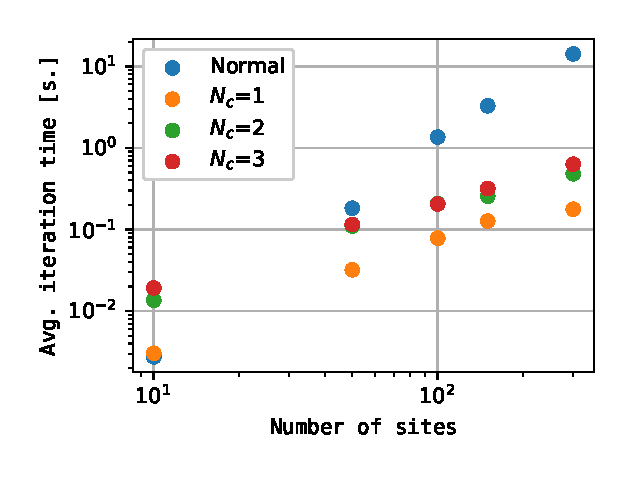
\includegraphics[width=0.6\textwidth]{figures/timing_plot}
	\caption{Timing of the methods compared to the system size in logarithmic scale. }
	\label{fig:timing_comp}
\end{figure}

In fig. \ref{fig:timing_comp} can it be observed that for small systems is the normal methods the fastest. Going merely half a magnitude up has it already become the slowest of the methods, and slows down at a considerable pace compared to the other methods. The time increases with nearly 3 magnitudes when the system size is increased by one magnitude. All the while the other methods all lie on the line where the time increases by one magnitude for each magnitude increase in system size. Limitation on the upper limit has been put by the hardware, so trends for larger systems than this cannot be observed. 
% section Comparison of the time taken (end)

\subsection{Error against NBM} % (fold)
\label{sub:error_against_nbm}

Define the norm here: square sum of the spatial energy gaps. Comparing two is the square of the diff between two at one site



% subsection Error against NBM (end)


\subsection{Critical temperature compared to chemical potential}
The system used here is $N = 30$ lattice sites, electron interaction strength $V=1.5t$, the temperature ranging from $0$ to $0.2t$ and the convergence threshold is set to $1e-8$. 

\begin{figure}[ht]
	\begin{subfigure}{0.5\textwidth}
	\begin{center}
		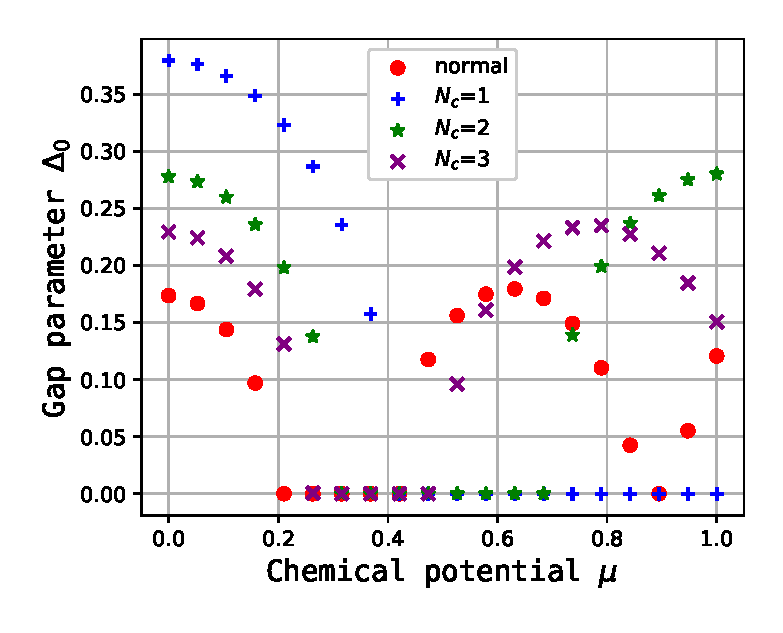
\includegraphics[width=\textwidth]{figures/delta0.eps}
	\caption{$\Delta_0$ plotted against the \\ chemical potential}
	\end{center}
	\end{subfigure}
	\begin{subfigure}{0.5\textwidth}
	\begin{center}
		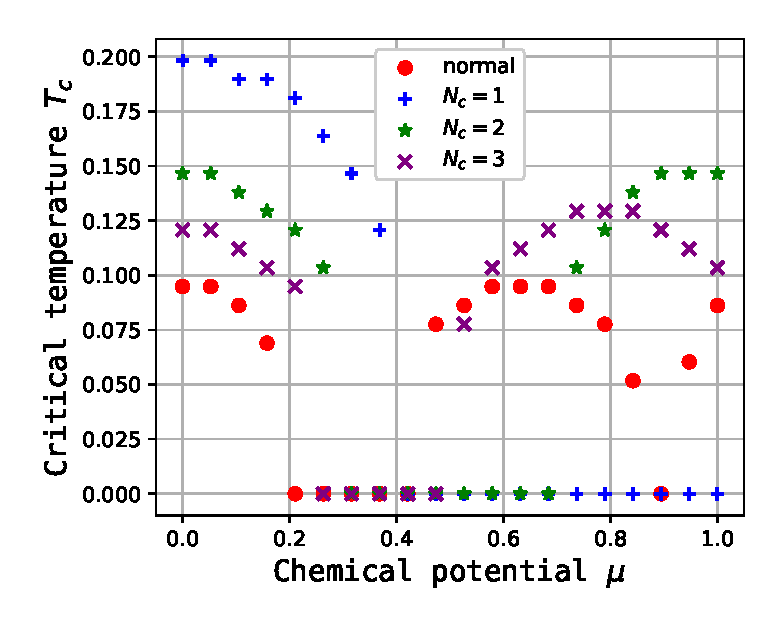
\includegraphics[width=\textwidth]{figures/critical_temperature.eps}
	\caption{Critical temperature $T_c$ plotted \\ against the chemical potential}
	\end{center}
	\end{subfigure}
	\caption{System with 30 sites where the chemical potential is varied. }
	\label{fig:chemical-potential-study}
\end{figure}

In fig. \ref{fig:chemical-potential-study} can we see four methods being used: one "normal" and three cluster methods with $N_c = 1, 2, 3$ respectively. We can observe that generally are $T_c$ and $\Delta_0$ related for the same methods. However, these is some pretty interesting behavior. For the normal method we see that for some specific $\mu$ can the system not enter a superconducting state, identified by the gap parameter being 0 at $T=0$. 



\section{Discussion}\label{sec:discussion}


\onecolumn
% ref
\bibliographystyle{plain} % We choose the "plain" reference style
\bibliography{refs} % Entries are in the refs.bib file

\end{document}

pdflatex: --aux-directory=build
bibtex: build/% -use-directory=build

